\documentclass{article}
\usepackage[a4paper, margin=2cm]{geometry}

\usepackage{amsmath}
\usepackage{amssymb}
\usepackage{mathtools}
\usepackage{amstext}
\usepackage{amsthm}
\usepackage{fancyhdr}
\usepackage{siunitx}
\usepackage{physics}

\usepackage{hyperref}

\usepackage{tikz}
\usetikzlibrary{patterns}
\usepackage{pgfplots}
\usetikzlibrary{arrows}
\usetikzlibrary{decorations.pathreplacing}



\usepackage{graphicx}
\usepackage{float}
\graphicspath{{figures/}} %Setting the graphicspath
\usepackage{float}
\usepackage{caption}
\usepackage{subcaption}
\usepackage{booktabs}

% To work with inkfigures
\usepackage{import}
\usepackage{pdfpages}
\usepackage{transparent}
\usepackage{xcolor}

\newcommand{\incfig}[2][1]{%
    \def\svgwidth{#1\columnwidth}
    \import{./figures/}{#2.pdf_tex}
}

\pdfsuppresswarningpagegroup=1

%\graphicspath{{figures/}}

\pagestyle{fancy}
\rhead{Alexandre Adam}
\lhead{PHY6669 -- Cosmologie \\ Alan Robinson}
\chead{Devoir 2}
\rfoot{\today}
\cfoot{\thepage}

\newcommand{\angstrom}{\textup{\AA}}
\numberwithin{equation}{section}
\renewcommand\thesubsection{\alph{subsection})}
\renewcommand\thesubsubsection{\Roman{subsubsection}}
\newcommand{\s}{\hspace{0.1cm}}

\newcommand{\pyoutput}[2]{#2}

% Astronomy
\DeclareSIUnit\parsec{pc}
\DeclareSIUnit\lightyear{ly}

\begin{document}
\section{Les distances en cosmologie}
\subsection{Distance angulaire}
On cherche le redshift $z$ où l'angle apparent d'un objet est à son minimum en supposant 
un univers dominé par la matière.

L'angle apparent d'un objet dépend de la taille que cette objet aurait au 
temps présent ($\ell(z)$) et de la distance 
comobile entre l'observateur et l'objet:
\begin{equation}\label{eq:AngleApparent} 
        \theta = \frac{\ell(z)}{\chi(z)}
\end{equation} 
Un objet de taille caractéristique $\ell$ (dans son référentiel, au temps 
où l'objet à émis la lumière observée) aura une taille assumée dans le référentiel 
de l'observateur égale à
\[
        \ell(z) = \frac{a_0}{a}\ell = (1 + z) \ell
\]
Pour un univers de poussière ($\Lambda = p = 0$), la distance comobile prend une forme 
analytique:
\begin{equation}\label{eq:ComovingDistanceDust} 
        \chi(z) = \frac{2 c}{H_0} \frac{\Omega_0 z + (\Omega_0 - 2)
        (\sqrt{\Omega_0 z + 1} - 1)}{\Omega_0^2(1 + z)}
\end{equation}
On peut donc déterminer un redshift où la taille atteint un maxima:
\begin{align*}
        \frac{d \theta}{d z} &= \frac{H_0 \ell}{2c} \frac{d }{d z} 
                \frac{\Omega_0^2(1 + z)^2}{\Omega_0 z + (\Omega_0 - 2) 
                (\sqrt{\Omega_0 z + 1} - 1)} \\
        &= \frac{\Omega_0^2 H_0 \ell}{2c} 
                \frac{2(1 + z) \left[ \Omega_0 z + (\Omega_0 - 2) 
                (\sqrt{\Omega_0 z + 1} - 1) \right] - 
        (1 + z)^{2} \left[ \Omega_0 + 
        \frac{1}{2}\frac{\Omega_0(\Omega_0 - 2) }{\sqrt{\Omega_0 z  + 1}}\right]}{
        (\Omega_0 z + (\Omega_0 - 2)(\sqrt{\Omega_0 z + 1} - 1))^{2}        
}
\end{align*}
Il s'avère qu'il est possible de résoudre analytiquement 
ce système seulement pour $\Omega_0 = 1$ (univers plat):
\begin{align*}
        \frac{d \theta}{d z}\bigg|_{\Omega_0=1} &= 0 \\
        \implies 2\left[ z -\sqrt{z + 1} + 1\right]
        &= (1 + z) \left[ 1 - \frac{1}{2\sqrt{z + 1}} \right] \\
        \implies 2(x^2 - x) &=  x^2(1 - \frac{1}{2x}), \hspace{1cm} \{x = \sqrt{z + 1} \} \\
        \implies x^2 - \frac{3x}{2} &=  0 \\
        \implies \sqrt{z + 1} &= \frac{3}{2}, \hspace{2.5cm} \{ z \geq 0 \implies x \not= 0 \} \\
        \implies \Aboxed{z &=  \frac{5}{4}}
\end{align*}
Il serait possible de faire un traitement perturbatoire pour $\Omega_0 = 1 \pm \epsilon$, 
$\epsilon \ll 1$, mais on trouve qu'une solution numérique sert mieux nos besoins. 
Les prochaines figures montrent le redshift où l'angle apparent est minimal pour une 
une densité totale $\Omega_0$ donnée.

\begin{figure}[H]
        \centering
        \begin{subfigure}[t]{0.52\textwidth}
                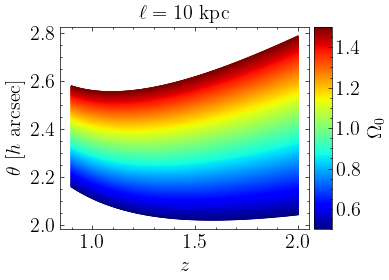
\includegraphics[width=\textwidth]{theta_z}
                \caption{Taille angulaire apparente d'un objet de distance 
                caractéristique $\ell$}
                \label{fig:theta_z}
        \end{subfigure}
        ~
        \begin{subfigure}[t]{0.45\textwidth}
                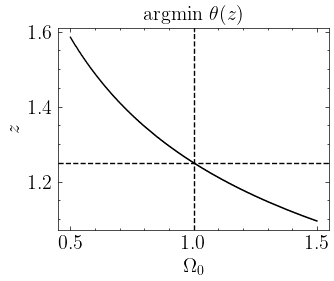
\includegraphics[width=\textwidth]{zmin} 
                \caption{Le redshift où $\theta$ est minimal
                        se comporte comme $\Omega_0^{-1}$ autour 
                        de la solution pour un univers plat.}
                \label{}
        \end{subfigure}
\end{figure}

\subsection{Le nombre total de galaxies dans l'univers}
Pour déterminer la densité de galaxie de l'univers à un temps donné, il est coutume de 
se référer à la fonction de Schechter pour mesurer la densité numérique de galaxies 
en fonction de leur distribution de masse:
\begin{equation}\label{eq:Schechter} 
        \phi(M) = b\phi^* \ln(10) \left[ 10^{b(M - M^{*})} \right]^{1 + \alpha} \exp \left\{ 
        -10^{b(M - M^{*})}\right\}
\end{equation} 
où $b=1$ pour la fonction de masse. En principe, $\alpha$, $M^{*}$ et $\phi^{*}$ doivent 
être ajusté sur les observations et peuvent dépendre de l'historique de formation 
des galaxies. En d'autres mots, ce sont des paramètres qui dépendent du redshift. On 
mesure $M$ en unité logarithmique de masse solaire:
\[
        M = \log \frac{M_{\text{gal}}}{M_\odot}
\]
La fonction de Schechter n'est valide que dans un interval de masses considérées. La borne 
inférieur choisie dans l'analyse de \cite{Conselice2016} est $M > 6$. Le meilleur fit sur les données 
pour la densité numérique intégrée sur le profile de Schechter $\phi_T$
\[
        \phi_T(z) = \int_{M_1}^{M_2} \phi(M, z) dM
\]
est \cite{Conselice2016}
\[
        \log \phi_T(t) = (-1.08 \pm 0.20) \log(t) - 0.26 \pm 0.06
\]
De sortes que le nombre total de galaxies dans l'univers visible, 
en supposant un modèle d'évolution
qui commence à $z = 6$ et la cosmologie du modèle $\Lambda \text{CDM}$ plat est
\begin{equation}\label{eq:NtotGal} 
        N_{\text{tot}} = \frac{c}{H_0} \int_{z=0}^{6} 
        \int_0^{4 \pi} \frac{(1 + z)^{2} D_A^{2}}{
        \sqrt{\Omega_{0m}(1 + z)^{3} + \Omega_{0\Lambda}}}
        \phi_T(t(z)) d\Omega dz
\end{equation} 
où $D_A$ est la distance angulaire en fonction de $z$
\begin{equation}\label{eq:DA} 
        D_A = \frac{1}{1 + z} \frac{1}{H_0}\int_0^{z} \frac{dz'}{\sqrt{\Omega_{0m}(1 + z')^{3} 
        + \Omega_{0\Lambda}}}
\end{equation} 
et
\begin{equation}\label{eq:t(z)} 
        t(z) = \frac{1}{H_0}\int_\infty^{z} \frac{(1 + z')^{-1} dz'}{
        \sqrt{\Omega_{0m}(1 + z')^{3} + \Omega_{0\Lambda}}}
\end{equation} 
Les paramètres du modèle cosmologique sont données dans la table suivante.
\begin{table}[H]
        \centering
        \begin{tabular}{ccc}
                \toprule
                $h$ & $\Omega_{0m}$ & $\Omega_\Lambda$ \\
                0.72 & 0.3 & 0.7 \\
                \bottomrule
                
        \end{tabular}
        \caption{}
        \label{tab:}
\end{table}
Le résultat de l'équation \eqref{eq:NtotGal} est 
\[
        \boxed{N_{\text{tot}} = 6.750 \times 10^{11}\, \text{galaxies}}
\]
En principe, il y a $N_{\text{tot}}$ galaxie observable dans l'univers visible.


\section{L'horizon}
L'horizon comobile est définie comme
\[
        \eta \equiv \int_0^t \frac{dt'}{a(t')}
\]
$(c = 1)$. La distance comobile entre deux points est définie comme
\[
        \chi(a) = \int_a^{1} \frac{da'}{a'^2 H(a')}
\]

\subsection{}
On cherche le redshift à partir duquel un miroir peut réfléchit la lumière du Big Bang 
vers la position d'un observateur de sortes que celui-ci reçoit cette lumière au temps 
$t_0$.
\begin{figure}[H]
        \centering
        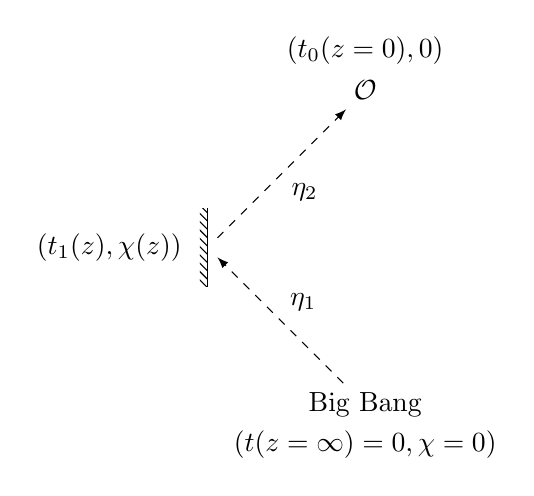
\begin{tikzpicture}
                \node (bb) at (0, 0) {Big Bang};
                \node at (0, -0.5) {$(t(z=\infty) = 0, \chi=0)$};
                \node (miroir) at (-2, 2) {};
                \node at (-3.25, 2) {$(t_1(z), \chi(z))$};
                \draw (-2, 1.5) -- (-2, 2.5); 
                \draw[pattern=north west lines, draw=none] (-2, 1.5) rectangle (-2.1, 2.5);
                \node (obs) at (0, 4) {$\mathcal{O}$};
                \node at (0, 4.5) {$(t_0(z=0), 0)$};
                \draw[-latex, dashed] (bb) -- (miroir) node [midway, above right] {$\eta_1$};
                \draw[-latex, dashed] (miroir) -- (obs) node [midway, below right] {$\eta_2$};
                %\draw[decorate, decoration={brace, amplitude=5pt, mirror}, xshift=0pt, yshift=0pt] 
                        %(-2, -1) -- (0, -1);
                %\node at (-1, -1.5) {$\chi(z)$};
        \end{tikzpicture}
        \caption{Illustration du problème}
        \label{fig:Numero2a}
\end{figure}

Par géométrie, les horizons comobiles $\eta_1$ et $\eta_2$ sont égales à la distance 
comobile $\chi(z)$ entre le miroir et l'observateur:
\[
        \chi(z) = \frac{1}{2} \left( \int_0^{t_1} \frac{dt}{a(t)} 
        + \int_{t_1}^{t_0} \frac{dt}{a(t)}\right)
\]
Pour un univers de poussière ($\Lambda=p=0$) plat ($\Omega_0=1$), les équations de 
Friedmann ont comme solution
\begin{align*}
        t(z) &=  t_0 (1 + z)^{-3/2} \\
        \implies dt &= -\frac{3}{2}t_0 (1 + z)^{-5/2}dz
\end{align*}
En remplaçant $a(z) = (1 + z)^{-1}$, dans l'intégrale de l'horizon comobile, on obtient
\[
        \chi(z) = \frac{1}{2} \int_\infty^{0} \left( - \frac{3}{2} \right)t_0
        (1 + z)^{-3/2} dz
\]
Ainsi,
\[
        \chi(z) = \frac{3}{2H_0}
\]
Du côté gauche, la distance comobile prend la forme
\[
        \chi(z) = \frac{2}{H_0}\left( 1 - \frac{1}{\sqrt{1 + z}} \right)      
\]
De sortes que 
\begin{align*}
        1 - \frac{1}{\sqrt{1 + z}} &=  \frac{3}{4} \\
        \implies \Aboxed{z &= 3} 
\end{align*}



\subsection{}
Dans un univers ouvert ($\kappa  = -1, \Omega < 1$) 
dominé par la matière ($\Lambda = p = 0$), les équations de Friedmann deviennent
\begin{align*}
        \dot{a}^{2} &=  \frac{8 \pi G \rho a^2}{3} - 1 \\
        \ddot{a} &=  -\frac{4\pi G \rho a}{3} \\
        d(\rho a^3) &=  0
\end{align*}
On introduit le paramètre de densité 
\[
        \Omega = \frac{\rho}{\rho_c}, \hspace{1cm} \rho_c = \frac{3H^2}{8 \pi G}
\]

\end{document}

